% tikzpic.tex
\documentclass[crop,tikz]{standalone}% 'crop' is the default for v1.0, before it was 'preview'
%\usetikzlibrary{...}% tikz package already loaded by 'tikz' option
\usepackage{pgfplots}
\pgfplotsset{width=10cm,compat=1.17,ytick style={draw=none},xtick style={draw=none}}

\begin{document}
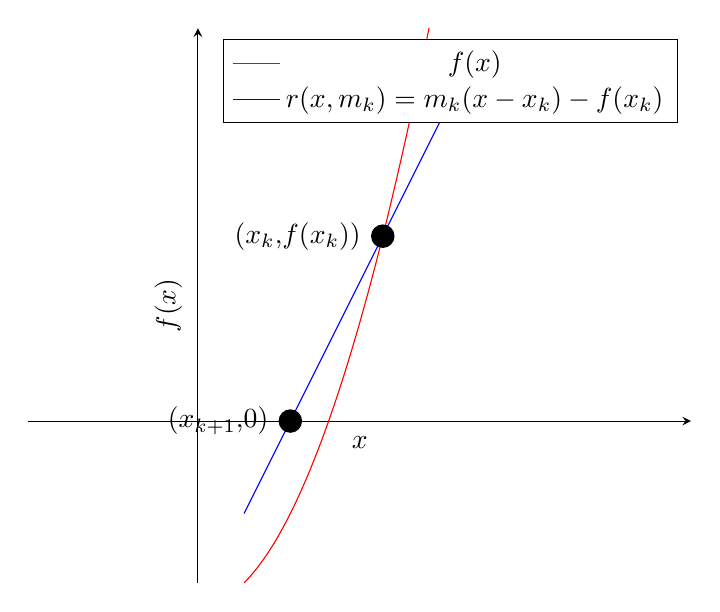
\begin{tikzpicture}
%%%
\begin{axis}[
    axis lines = left,
    xlabel = \(x\),
    ylabel = {\(f(x)\)},
    grid=major, % Display a grid
    grid style={dashed,gray!30}, % Set the
    axis equal,
    axis x line*=middle,
    axis y line*=middle,
    xtick=\empty,
    ytick=\empty,
]
% f(x)
\addplot [
    domain=0.5:2.5, 
    samples=100, 
    color=red,
]
{x^2 - 2};
\addlegendentry{\(f(x)\)}
\addplot [
    domain=0.5:3, 
    samples=100, 
    color=blue,
    ]
    {2*x-2};
\addlegendentry{\(r(x, m_k) = m_k (x - x_k) - f(x_k) \)}
%\addplot coordinates {(2,2)};
\node[label={180:{($x_k$,$f(x_k)$)}},circle,fill,,inner sep=3pt] at (axis cs:2,2) {};
%\node[label={180:{($x_{k+1}$,0)}},circle,fill,inner sep=3pt] at (axis cs:1.414,0) {};
\node[label={180:{($x_{k+1}$,0)}},circle,fill,inner sep=3pt] at (axis cs:1,0) {};
\end{axis}
%%%
\end{tikzpicture}
\end{document}